\documentclass{beamer}
\usepackage{amsmath,graphics}
\usepackage{amssymb}

\usetheme{default}
\usepackage{xcolor}

\definecolor{solarizedBase03}{HTML}{002B36}
\definecolor{solarizedBase02}{HTML}{073642}
\definecolor{solarizedBase01}{HTML}{586e75}
\definecolor{solarizedBase00}{HTML}{657b83}
\definecolor{solarizedBase0}{HTML}{839496}
\definecolor{solarizedBase1}{HTML}{93a1a1}
\definecolor{solarizedBase2}{HTML}{EEE8D5}
\definecolor{solarizedBase3}{HTML}{FDF6E3}
\definecolor{solarizedYellow}{HTML}{B58900}
\definecolor{solarizedOrange}{HTML}{CB4B16}
\definecolor{solarizedRed}{HTML}{DC322F}
\definecolor{solarizedMagenta}{HTML}{D33682}
\definecolor{solarizedViolet}{HTML}{6C71C4}
%\definecolor{solarizedBlue}{HTML}{268BD2}
\definecolor{solarizedBlue}{HTML}{134676}
\definecolor{solarizedCyan}{HTML}{2AA198}
\definecolor{solarizedGreen}{HTML}{859900}
\definecolor{myBlue}{HTML}{162DB0}%{261CA4}
\setbeamercolor*{item}{fg=myBlue}
\setbeamercolor{normal text}{fg=solarizedBase03, bg=solarizedBase3}
\setbeamercolor{alerted text}{fg=myBlue}
\setbeamercolor{example text}{fg=myBlue, bg=solarizedBase3}
\setbeamercolor*{frametitle}{fg=solarizedRed}
\setbeamercolor*{title}{fg=solarizedRed}
\setbeamercolor{block title}{fg=myBlue, bg=solarizedBase3}
\setbeameroption{hide notes}
\setbeamertemplate{note page}[plain]
\beamertemplatenavigationsymbolsempty
\usefonttheme{professionalfonts}
\usefonttheme{serif}

\usepackage{fourier}

\def\vec#1{\mathchoice{\mbox{\boldmath$\displaystyle#1$}}
{\mbox{\boldmath$\textstyle#1$}}
{\mbox{\boldmath$\scriptstyle#1$}}
{\mbox{\boldmath$\scriptscriptstyle#1$}}}
\definecolor{OwnGrey}{rgb}{0.560,0.000,0.000} % #999999
\definecolor{OwnBlue}{rgb}{0.121,0.398,0.711} % #1f64b0
\definecolor{red4}{rgb}{0.5,0,0}
\definecolor{blue4}{rgb}{0,0,0.5}
\definecolor{Blue}{rgb}{0,0,0.66}
\definecolor{LightBlue}{rgb}{0.9,0.9,1}
\definecolor{Green}{rgb}{0,0.5,0}
\definecolor{LightGreen}{rgb}{0.9,1,0.9}
\definecolor{Red}{rgb}{0.9,0,0}
\definecolor{LightRed}{rgb}{1,0.9,0.9}
\definecolor{White}{gray}{1}
\definecolor{Black}{gray}{0}
\definecolor{LightGray}{gray}{0.8}
\definecolor{Orange}{rgb}{0.1,0.2,1}
\setbeamerfont{sidebar right}{size=\scriptsize}
\setbeamercolor{sidebar right}{fg=Black}

\renewcommand{\emph}[1]{{\textcolor{solarizedRed}{\itshape #1}}}

\newcommand\cA{\mathcal A}
\newcommand\cB{\mathcal B}
\newcommand\cC{\mathcal C}
\newcommand\cD{\mathcal D}
\newcommand\cE{\mathcal E}
\newcommand\cF{\mathcal F}
\newcommand\cG{\mathcal G}
\newcommand\cH{\mathcal H}
\newcommand\cI{\mathcal I}
\newcommand\cJ{\mathcal J}
\newcommand\cK{\mathcal K}
\newcommand\cL{\mathcal L}
\newcommand\cM{\mathcal M}
\newcommand\cN{\mathcal N}
\newcommand\cO{\mathcal O}
\newcommand\cP{\mathcal P}
\newcommand\cQ{\mathcal Q}
\newcommand\cR{\mathcal R}
\newcommand\cS{\mathcal S}
\newcommand\cT{\mathcal T}
\newcommand\cU{\mathcal U}
\newcommand\cV{\mathcal V}
\newcommand\cW{\mathcal W}
\newcommand\cX{\mathcal X}
\newcommand\cY{\mathcal Y}
\newcommand\cZ{\mathcal Z}

\newcommand\fA{\mathfrak A}
\newcommand\fB{\mathfrak B}
\newcommand\fC{\mathfrak C}
\newcommand\fD{\mathfrak D}
\newcommand\fE{\mathfrak E}
\newcommand\fF{\mathfrak F}
\newcommand\fG{\mathfrak G}
\newcommand\fH{\mathfrak H}
\newcommand\fI{\mathfrak I}
\newcommand\fJ{\mathfrak J}
\newcommand\fK{\mathfrak K}
\newcommand\fL{\mathfrak L}
\newcommand\fM{\mathfrak M}
\newcommand\fN{\mathfrak N}
\newcommand\fO{\mathfrak O}
\newcommand\fP{\mathfrak P}
\newcommand\fQ{\mathfrak Q}
\newcommand\fR{\mathfrak R}
\newcommand\fS{\mathfrak S}
\newcommand\fT{\mathfrak T}
\newcommand\fU{\mathfrak U}
\newcommand\fV{\mathfrak V}
\newcommand\fW{\mathfrak W}
\newcommand\fX{\mathfrak X}
\newcommand\fY{\mathfrak Y}
\newcommand\fZ{\mathfrak Z}

\newcommand\fa{\mathfrak a}
\newcommand\fb{\mathfrak b}
\newcommand\fc{\mathfrak c}
\newcommand\fd{\mathfrak d}
\newcommand\fe{\mathfrak e}
\newcommand\ff{\mathfrak f}
\newcommand\fg{\mathfrak g}
\newcommand\fh{\mathfrak h}
%\newcommand\fi{\mathfrak i}
\newcommand\fj{\mathfrak j}
\newcommand\fk{\mathfrak k}
\newcommand\fl{\mathfrak l}
\newcommand\fm{\mathfrak m}
\newcommand\fn{\mathfrak n}
\newcommand\fo{\mathfrak o}
\newcommand\fp{\mathfrak p}
\newcommand\fq{\mathfrak q}
\newcommand\fr{\mathfrak r}
\newcommand\fs{\mathfrak s}
\newcommand\ft{\mathfrak t}
\newcommand\fu{\mathfrak u}
\newcommand\fv{\mathfrak v}
\newcommand\fw{\mathfrak w}
\newcommand\fx{\mathfrak x}
\newcommand\fy{\mathfrak y}
\newcommand\fz{\mathfrak z}

\newcommand\vA{\vec A}
\newcommand\vB{\vec B}
\newcommand\vC{\vec C}
\newcommand\vD{\vec D}
\newcommand\vE{\vec E}
\newcommand\vF{\vec F}
\newcommand\vG{\vec G}
\newcommand\vH{\vec H}
\newcommand\vI{\vec I}
\newcommand\vJ{\vec J}
\newcommand\vK{\vec K}
\newcommand\vL{\vec L}
\newcommand\vM{\vec M}
\newcommand\vN{\vec N}
\newcommand\vO{\vec O}
\newcommand\vP{\vec P}
\newcommand\vQ{\vec Q}
\newcommand\vR{\vec R}
\newcommand\vS{\vec S}
\newcommand\vT{\vec T}
\newcommand\vU{\vec U}
\newcommand\vV{\vec V}
\newcommand\vW{\vec W}
\newcommand\vX{\vec X}
\newcommand\vY{\vec Y}
\newcommand\vZ{\vec Z}

\newcommand\va{\vec a}
\newcommand\vb{\vec b}
\newcommand\vc{\vec c}
\newcommand\vd{\vec d}
\newcommand\ve{\vec e}
\newcommand\vf{\vec f}
\newcommand\vg{\vec g}
\newcommand\vh{\vec h}
\newcommand\vi{\vec i}
\newcommand\vj{\vec j}
\newcommand\vk{\vec k}
\newcommand\vl{\vec l}
\newcommand\vm{\vec m}
\newcommand\vn{\vec n}
\newcommand\vo{\vec o}
\newcommand\vp{\vec p}
\newcommand\vq{\vec q}
\newcommand\vr{\vec r}
\newcommand\vs{\vec s}
\newcommand\vt{\vec t}
\newcommand\vu{\vec u}
\newcommand\vv{\vec v}
\newcommand\vw{\vec w}
\newcommand\vx{\vec x}
\newcommand\vy{\vec y}
\newcommand\vz{\vec z}

\renewcommand\AA{\mathbb A}
\newcommand\NN{\mathbb N}
\newcommand\ZZ{\mathbb Z}
\newcommand\PP{\mathbb P}
\newcommand\QQ{\mathbb Q}
\newcommand\RR{\mathbb R}
\renewcommand\SS{\mathbb S}
\newcommand\CC{\mathbb C}

\newcommand{\ord}{\mathrm{ord}}
\newcommand{\id}{\mathrm{id}}
\newcommand{\pr}{\mathrm{P}}
\newcommand{\Vol}{\mathrm{vol}}
\newcommand\norm[1]{\left\|{#1}\right\|} 
\newcommand\sign{\mathrm{sign}}
\newcommand{\eps}{\varepsilon}
\newcommand{\abs}[1]{\left|#1\right|}
\newcommand\bc[1]{\left({#1}\right)} 
\newcommand\cbc[1]{\left\{{#1}\right\}} 
\newcommand\bcfr[2]{\bc{\frac{#1}{#2}}} 
\newcommand{\bck}[1]{\left\langle{#1}\right\rangle} 
\newcommand\brk[1]{\left\lbrack{#1}\right\rbrack} 
\newcommand\scal[2]{\bck{{#1},{#2}}} 
\newcommand{\vecone}{\mathbb{1}}
\newcommand{\tensor}{\otimes}
\newcommand{\diag}{\mathrm{diag}}
\newcommand{\ggt}{\mathrm{ggT}}
\newcommand{\kgv}{\mathrm{kgV}}
\newcommand{\trans}{\top}

\newcommand{\Karonski}{Karo\'nski}
\newcommand{\Erdos}{Erd\H{o}s}
\newcommand{\Renyi}{R\'enyi}
\newcommand{\Lovasz}{Lov\'asz}
\newcommand{\Juhasz}{Juh\'asz}
\newcommand{\Bollobas}{Bollob\'as}
\newcommand{\Furedi}{F\"uredi}
\newcommand{\Komlos}{Koml\'os}
\newcommand{\Luczak}{\L uczak}
\newcommand{\Kucera}{Ku\v{c}era}
\newcommand{\Szemeredi}{Szemer\'edi}

\renewcommand{\ae}{\"a}
\renewcommand{\oe}{\"o}
\newcommand{\ue}{\"u}
\newcommand{\Ae}{\"A}
\newcommand{\Oe}{\"O}
\newcommand{\Ue}{\"U}

\newcommand{\im}{\mathrm{im}}

\newcommand{\mytitle}{Lineare Abbildungen}

\title[Linadi]{\mytitle}
\author[Amin Coja-Oghlan]{Amin Coja-Oghlan}
\institute[Frankfurt]{JWGUFFM}
\date{}

\begin{document}

\frame[plain]{\titlepage}

\begin{frame}\frametitle{\mytitle}
	\begin{block}{Definition}
		Seien $m,n\in\NN$.
		Eine Abbildung $f:\RR^n\to\RR^m$ hei\ss t \emph{linear}, wenn
		\begin{align*}
			f(u+v)&=f(u)+f(v)&&\mbox{f\ue r alle }u,v\in\RR^n\mbox{ und}\\
			f(c\cdot u)&=c\cdot f(u)&&\mbox{f\ue r alle }c\in\RR,\,u\in\RR^n.
		\end{align*}
	\end{block}
\end{frame}

\begin{frame}\frametitle{\mytitle}
	\begin{block}{Proposition}
		Seien $m,n\in\NN$.
		Eine Abbildung $f:\RR^n\to\RR^m$ ist genau dann linear, wenn es eine $m\times n$-Matrix $A$ gibt, so da\ss\
		\begin{align*}
			f(u)&=A\cdot u&&\mbox{f\ue r alle }u\in\RR^n.
		\end{align*}
		Wir nennen $A$ die \emph{darstellende Matrix} von $f$.
	\end{block}
\end{frame}

\begin{frame}\frametitle{\mytitle}
	\hfill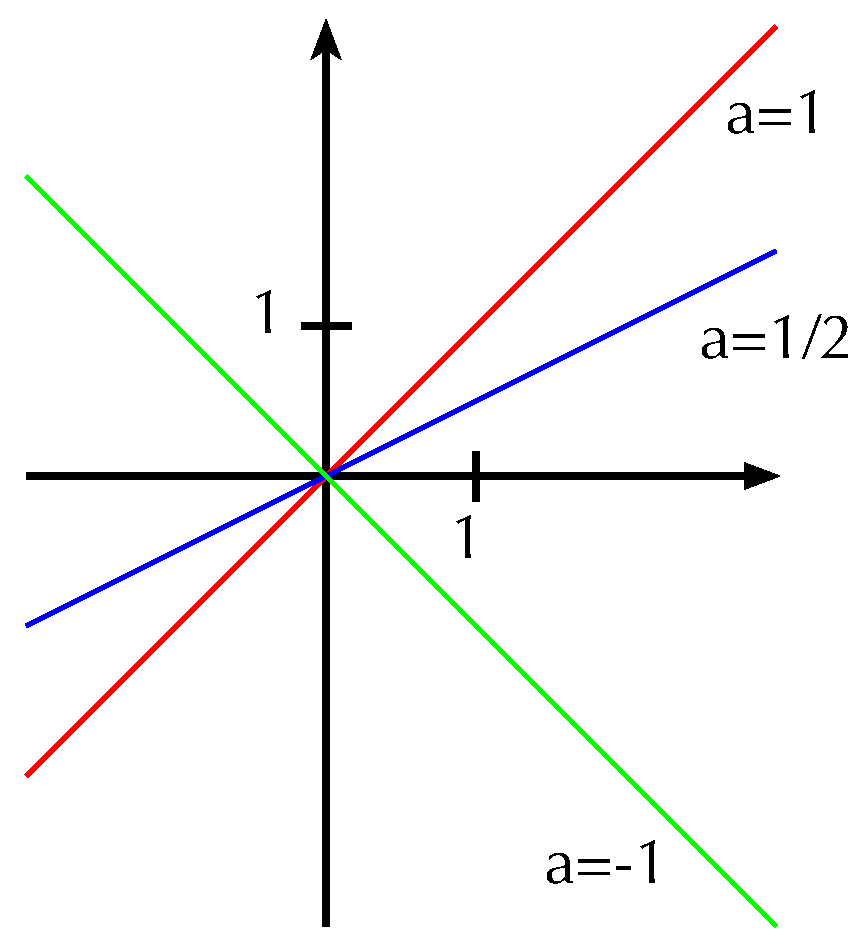
\includegraphics[height=30mm]{pics/linear1d.pdf}
	\begin{block}{Beispiele}
	\begin{itemize}
	\item Im Fall $m=n=1$ sind lineare Abbildungen von der Form
		\begin{align*}
			f:\RR&\to\RR&u\mapsto a\cdot u&&\mbox{f\ue r ein }a\in\RR.
		\end{align*}
		Der Graph einer solchen Funktion ist eine Gerade.
	\item In der Abbildung sind die Graphen eingezeichnet f\ue r $a\in\{1,1/2,-1\}$.
	\end{itemize}
	\end{block}
\end{frame}

\begin{frame}\frametitle{\mytitle}
	\hfill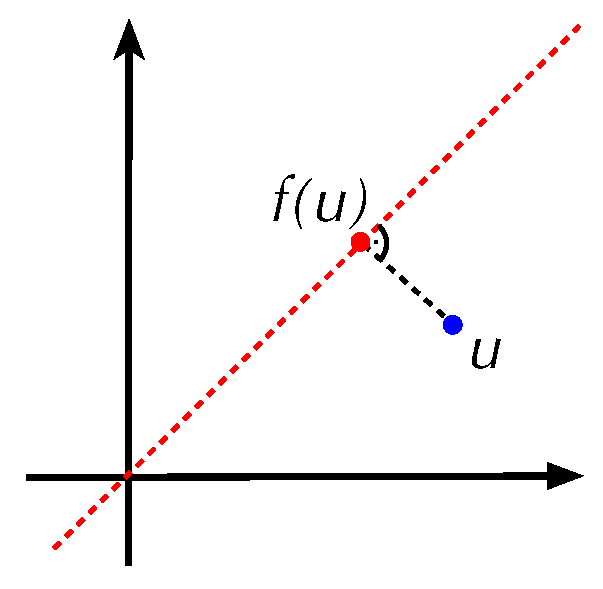
\includegraphics[height=30mm]{pics/linear2d.pdf}
	\begin{block}{Beispiele}
	\begin{itemize}
	\item Im Fall $m=1$, $n\geq1$ sind lineare Abbildungen von der Form
		\begin{align*}
			f:\RR^n&\to\RR&u\mapsto a^\trans u&&\mbox{f\ue r ein }a\in\RR^n.
		\end{align*}
	\item Beispielsweise ist 
		\begin{align*}
			f:u=\binom{u_1}{u_2}\in\RR^2&\mapsto\binom{1/\sqrt 2}{1/\sqrt 2}^\trans u=\frac{u_1+u_2}{\sqrt 2}
		\end{align*}
		geometrisch die Projektion auf die Winkelhalbierende.
	\end{itemize}
	\end{block}
\end{frame}

\begin{frame}\frametitle{\mytitle}
	\vspace{-8mm}
	\hfill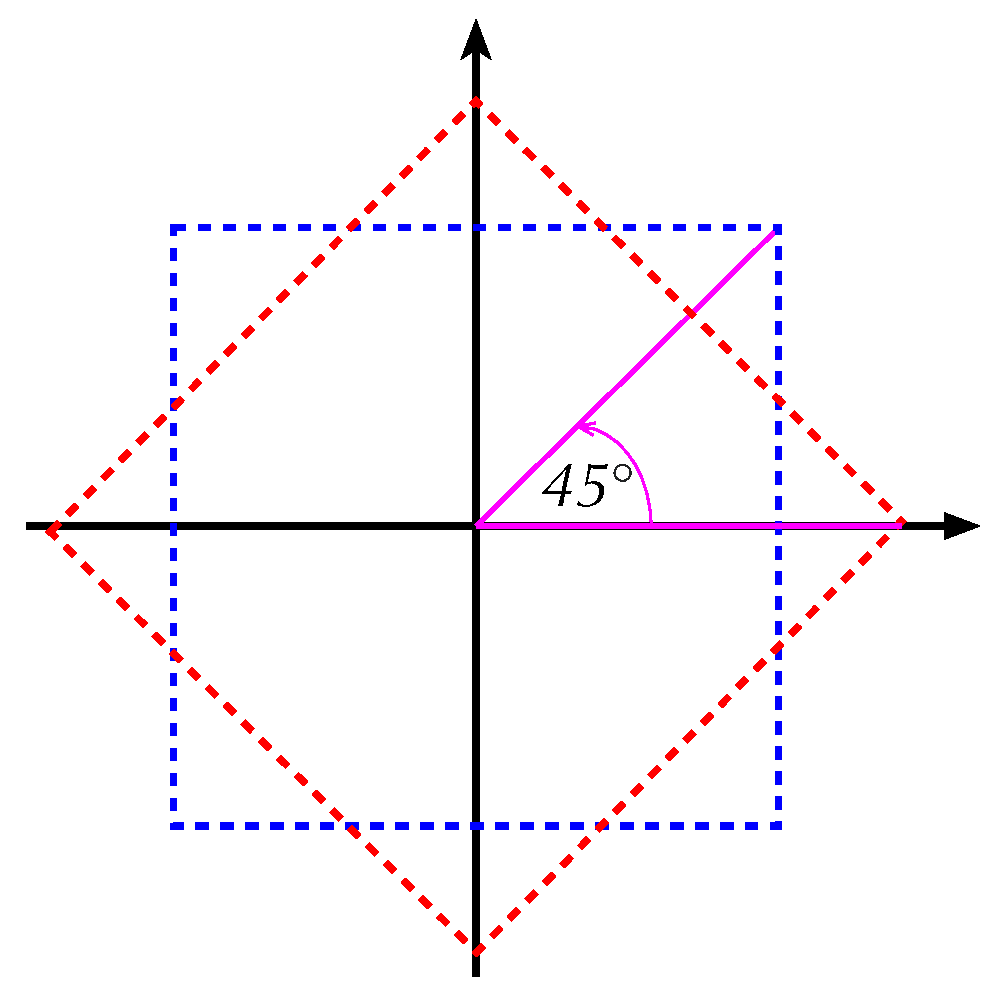
\includegraphics[height=40mm]{pics/rotation.pdf}
	\begin{block}{Beispiele}
	\begin{itemize}
	\item Lineare Abbildungen mit $n=m=2$ haben die Form
		\begin{align*}
			f:\RR^2&\to\RR^2&u\mapsto \begin{pmatrix}a_{11}&a_{12}\\a_{21}&a_{22}\end{pmatrix}\cdot\binom{u_1}{u_2}=\binom{a_{11}u_1+a_{12}u_2}{a_{21}u_1+a_{22}u_2}
		\end{align*}
	\item Eine konkretes Beispiel ist eine Drehung um $45^\circ$:  
		\begin{align*}
			f(u)&=\begin{pmatrix}\sqrt 2/2&-\sqrt 2/2\\\sqrt 2/2&\sqrt 2/2\end{pmatrix}\cdot\binom{u_1}{u_2}
		\end{align*}
	\end{itemize}
	\end{block}
\end{frame}

\begin{frame}\frametitle{\mytitle}
	\vspace{-8mm}
	\hfill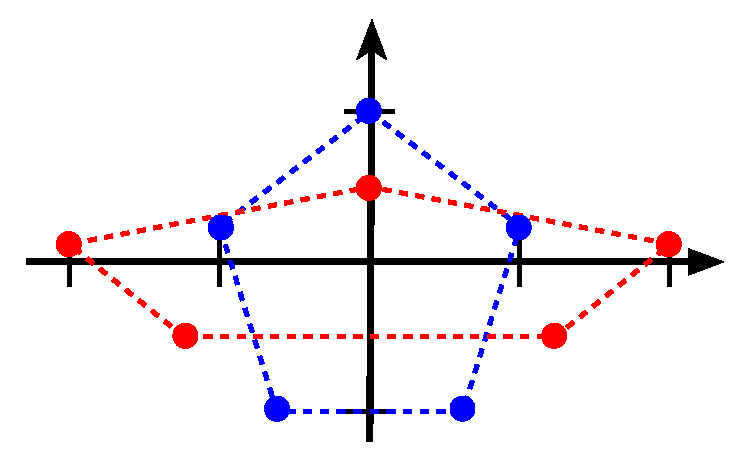
\includegraphics[height=40mm]{pics/stretch.pdf}
	\begin{block}{Beispiele}
	\begin{itemize}
	\item Diagonalmatrizen spielen eine besondere Rolle.
	\item Positive Diagonaleeintr\ae ge stauchen/strecken in Richtung der entsprechenden Achse.
	\item Konkretes Beispiel:
		\begin{align*}
			u&\mapsto\begin{pmatrix}2&0\\0&1/2\end{pmatrix}\cdot\binom{u_1}{u_2}=\binom{2u_1}{u_2/2}
		\end{align*}
	\end{itemize}
	\end{block}
\end{frame}

\begin{frame}\frametitle{\mytitle}
	\vspace{-8mm}
	\hfill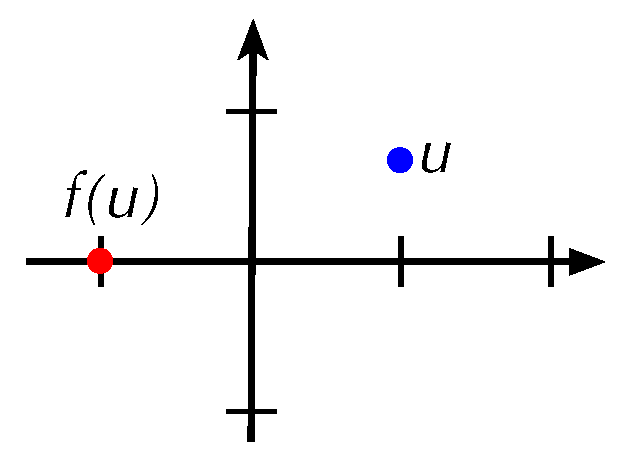
\includegraphics[height=40mm]{pics/reflect.pdf}
	\begin{block}{Beispiele}
	\begin{itemize}
	\item Diagonalmatrizen spielen eine besondere Rolle.
	\item Negative Diagonaleeintr\ae ge spiegeln.
	\item Null-Diagonaleeintr\ae ge projizieren die entsprechende Richtung heraus.
	\item Konkretes Beispiel:
		\begin{align*}
			u&\mapsto\begin{pmatrix}-1&0\\0&0\end{pmatrix}\cdot\binom{u_1}{u_2}=\binom{-u_1}0
		\end{align*}
	\end{itemize}
	\end{block}
\end{frame}

\begin{frame}\frametitle{\mytitle}
	\begin{block}{Addition von linearen Abbildungen}
		\begin{itemize}
			\item Seien $f,g:\RR^n\to\RR^m$ lineare Abbildungen.
			\item Seien $A,B$ ihre darstellenden Matrizen, d.h.\
				\begin{align*}
					f(u)&=Au&g(u)&=Bu
				\end{align*}
			\item Dann ist auch $f+g:\RR^n\to\RR^m$, $u\mapsto f(u)+g(u)$ linear.
			\item Die darstellende Matrix ist $A+B$, d.h.\
				\begin{align*}
					(f+g)(u)&=(A+B)u
				\end{align*}
		\end{itemize}
	\end{block}
\end{frame}

\begin{frame}\frametitle{\mytitle}
	\begin{block}{Multiplikation mit einem Skalar}
		\begin{itemize}
			\item Sei $f:\RR^n\to\RR^m$ eine lineare Abbildung.
			\item Sei $c\in\RR$.
			\item Dann ist auch
				\begin{align*}
					c\cdot f&:\RR^n\to\RR^m&u&\mapsto c\cdot f(u)
				\end{align*}
				linear.
			\item Wenn $A$ die darstellende Matrix von $f$ ist, so ist $c\cdot A$ die darstellende Matrix von $c\cdot f$.
		\end{itemize}
	\end{block}
\end{frame}

\begin{frame}\frametitle{\mytitle}
	\begin{block}{Komposition von Abbildungen}
		\begin{itemize}
			\item Sei $f:\RR^n\to\RR^m$ eine lineare Abbildung.
			\item Sei $g:\RR^m\to\RR^\ell$ eine weitere lineare Abbildung.
			\item Dann ist auch
				\begin{align*}
					g\circ f&:\RR^n\to\RR^\ell&u&\mapsto g(f(u))
				\end{align*}
				linear.
			\item Ist $A$ die darstellende Matrix von $f$ und $B$ die darstellende Matrix von $g$, so ist $B\cdot A$ die darstellende Matrix von $g\circ f$, also
				\begin{align*}
					g\circ f(u)&=B\cdot A\cdot u
				\end{align*}
		\end{itemize}
	\end{block}
\end{frame}

\begin{frame}\frametitle{\mytitle}
	\begin{block}{Das Bild}
		\begin{itemize}
			\item Sei $f:\RR^n\to\RR^m$ eine lineare Abbildung.
			\item Das \emph{Bild} von $f$ ist definiert als
				\begin{align*}
					\im(f)&=\cbc{f(u):u\in\RR^n}.
				\end{align*}
			\item Das Bild einer $m\times n$-Matrix $A$ ist definiert als
				\begin{align*}
					\im(A)&=\cbc{Au:u\in\RR^n}.
				\end{align*}
		\end{itemize}
	\end{block}
\end{frame}

\begin{frame}\frametitle{\mytitle}
	\begin{block}{Beispiel}
		\begin{itemize}
			\item Die Matrix $\id_n$ stellt die Abbildung
				\begin{align*}
					u\in\RR^n\mapsto \id_n u=u\in\RR^n
				\end{align*}
				dar.
			\item Diese bildet also jeden Vektor auf sich selbst ab.
			\item Das Bild dieser Abbildung ist $\RR^n$.
		\end{itemize}
	\end{block}
\end{frame}

\begin{frame}\frametitle{\mytitle}
	\begin{block}{Beispiel}
		\begin{itemize}
			\item Die lineare Abbildung 
				\begin{align*}
					u\in\RR^2\mapsto\begin{pmatrix}-1&0\\0&0\end{pmatrix}u\in\RR^2
				\end{align*}
				hat das Bild
				\begin{align*}
					\im\begin{pmatrix}-1&0\\0&0\end{pmatrix}&=\cbc{\begin{pmatrix}-1&0\\0&0\end{pmatrix}u:\in\RR^2}=\cbc{\binom{x}0:x\in\RR}
				\end{align*}
			\item Geometrisch gesprochen ist das Bild also die $x$-Achse.
		\end{itemize}
	\end{block}
\end{frame}

\begin{frame}\frametitle{\mytitle}
	\begin{block}{Beispiel}
		\begin{itemize}
			\item Die lineare Abbildung 
				\begin{align*}
					u\in\RR^2\mapsto\begin{pmatrix}1&2\\0&-1\\0&0\end{pmatrix}u\in\RR^3
				\end{align*}
				hat das Bild
				\begin{align*}
					\im\begin{pmatrix}1&2\\0&-1\\0&0\end{pmatrix}&
					=\cbc{\begin{pmatrix}u_1+2u_2\\-u_2\\0\end{pmatrix}:u_1,u_2\in\RR}	=\cbc{\begin{pmatrix}x\\y\\0\end{pmatrix}:x,y\in\RR}
				\end{align*}
			\item Geometrisch handelt es sich um die $xy$-Ebene.
		\end{itemize}
	\end{block}
\end{frame}

\begin{frame}\frametitle{\mytitle}
	\begin{block}{Der Kern}
		\begin{itemize}
			\item Der Kern einer linearen Abbildung $f:\RR^n\to\RR^m$ ist definiert als
				\begin{align*}
					\ker(f)&=\cbc{u\in\RR^n:f(u)=0}
				\end{align*}
			\item Der Kern einer $m\times n$-Matrix $A$ ist definiert als
\begin{align*}
					\ker(A)&=\cbc{u\in\RR^n:Au=0}
				\end{align*}
			\item F\ue r alle $f,A$ gilt
				\begin{align*}
					0\in\ker(f)\qquad 0\in\ker(A)
				\end{align*}
		\end{itemize}
	\end{block}
\end{frame}

\begin{frame}\frametitle{\mytitle}
	\begin{block}{Beispiel}
		\begin{itemize}
			\item Die Matrix $\id_n$ stellt die Abbildung
				\begin{align*}
					u\in\RR^n\mapsto \id_n u=u\in\RR^n
				\end{align*}
				dar.
			\item Der Kern dieser Abbildung ist $\ker(\id_n)=\cbc0$.
		\end{itemize}
	\end{block}
\end{frame}

\begin{frame}\frametitle{\mytitle}
	\begin{block}{Beispiel}
		\begin{itemize}
			\item Die lineare Abbildung 
				\begin{align*}
					u\in\RR^2\mapsto\begin{pmatrix}-1&0\\0&0\end{pmatrix}u\in\RR^2
				\end{align*}
				hat den Kern
				\begin{align*}
					\ker\begin{pmatrix}-1&0\\0&0\end{pmatrix}&=\cbc{\binom 0y:y\in\RR}.
				\end{align*}
		\end{itemize}
	\end{block}
\end{frame}

\begin{frame}\frametitle{\mytitle}
	\begin{block}{Beispiel}
		\begin{itemize}
			\item Die lineare Abbildung 
				\begin{align*}
					u\in\RR^2\mapsto\begin{pmatrix}1&2\\0&-1\\0&0\end{pmatrix}u\in\RR^3
				\end{align*}
				hat Kern
				\begin{align*}
					\ker\begin{pmatrix}1&2\\0&-1\\0&0\end{pmatrix}&
					=\cbc{\binom{u_1}{u_2}\in\RR^2:u_1+2u_2=-u_2=0}=\cbc{0}.
				\end{align*}
		\end{itemize}
	\end{block}
\end{frame}

\begin{frame}\frametitle{\mytitle}
	\begin{block}{Zusammenfassung}
		\begin{itemize}
			\item Eine lineare Abbildung $f:\RR^n\to\RR^m$ kann durch eine $m\times n$-Matrix $A$ dargestellt werden, so da\ss\
				\begin{align*}
					f(u)&=A\cdot u
				\end{align*}
			\item Umgekehrt induziert jede $m\times n$-Matrix $A$ die lineare Abbildung $u\mapsto Au$.
			\item Wir haben den Kern und das Bild linearer Abbildungen kennengelernt.
			\item \emph{Frage:} wie bestimmt man den Kern und das Bild?
		\end{itemize}
	\end{block}
\end{frame}

\end{document}
